
\documentclass[10pt]{article}

\usepackage{graphicx}
\usepackage{amsmath,amsfonts,amssymb}

\usepackage{hyperref}  % for urls and hyperlinks


\setlength{\textwidth}{6.2in}
\setlength{\oddsidemargin}{0.3in}
\setlength{\evensidemargin}{0in}
\setlength{\textheight}{8.9in}
\setlength{\voffset}{-1in}
\setlength{\headsep}{26pt}
\setlength{\parindent}{0pt}
\setlength{\parskip}{5pt}



% a few handy macros

\newcommand\matlab{{\sc matlab}}
\newcommand{\goto}{\rightarrow}
\newcommand{\bigo}{{\mathcal O}}
\newcommand{\half}{\frac{1}{2}}
%\newcommand\implies{\quad\Longrightarrow\quad}
\newcommand\reals{{{\rm l} \kern -.15em {\rm R} }}
\newcommand\complex{{\raisebox{.043ex}{\rule{0.07em}{1.56ex}} \hskip -.35em {\rm C}}}


% macros for matrices/vectors:

% matrix environment for vectors or matrices where elements are centered
\newenvironment{mat}{\left[\begin{array}{ccccccccccccccc}}{\end{array}\right]}
\newcommand\bcm{\begin{mat}}
\newcommand\ecm{\end{mat}}

% matrix environment for vectors or matrices where elements are right justifvied
\newenvironment{rmat}{\left[\begin{array}{rrrrrrrrrrrrr}}{\end{array}\right]}
\newcommand\brm{\begin{rmat}}
\newcommand\erm{\end{rmat}}

% for left brace and a set of choices
\newenvironment{choices}{\left\{ \begin{array}{ll}}{\end{array}\right.}
\newcommand\when{&\text{if~}}
\newcommand\otherwise{&\text{otherwise}}
% sample usage:
%  \delta_{ij} = \begin{choices} 1 \when i=j, \\ 0 \otherwise \end{choices}


% for labeling and referencing equations:
\newcommand{\eql}{\begin{equation}\label}
\newcommand{\eqn}[1]{(\ref{#1})}
% can then do
%  \eql{eqnlabel}
%  ...
%  \end{equation}
% and refer to it as equation \eqn{eqnlabel}.  


% some useful macros for finite difference methods:
\newcommand\unp{U^{n+1}}
\newcommand\unm{U^{n-1}}

% for chemical reactions:
\newcommand{\react}[1]{\stackrel{K_{#1}}{\rightarrow}}
\newcommand{\reactb}[2]{\stackrel{K_{#1}}{~\stackrel{\rightleftharpoons}
   {\scriptstyle K_{#2}}}~}

% Parts:

% set enumerate to give parts a, b, c, ...  rather than numbers 1, 2, 3...
\renewcommand{\theenumi}{\alph{enumi}}
\renewcommand{\labelenumi}{(\theenumi)}

% set second level enumerate to give parts i, ii, iii, iv, etc.
\renewcommand{\theenumii}{\roman{enumii}}
\renewcommand{\labelenumii}{(\theenumii)}




\begin{document}

% header:
\hfill \vbox{
\hbox{AMath 584 / Math 584}
\hbox{Homework \#1}
\hbox{Due 11:00pm PDT}
\hbox{Tuesday, October 11, 2016}
}


\vskip 0.5cm

{\bf Name:}   Your Name Here

{\bf Netid:}  Your NetID Here

\vskip 0.5cm

%--------------------------------------------------------------------------
\vskip 1cm
\hrule
{\bf Problem 1.}
Exercise 1.1 in Trefethen and Bau.
Note for example that part (a) is accomplished by multiplying $B$ on the
right by the matrix
\[
C_1 = \bcm 2&0&0&0\\ 0&1&0&0\\ 0&0&1&0\\ 0&0&0&1\ecm
\]
You can write out analogous matrices for each step and then write the
required product of these matrices.  Make sure to write them
{\em in the correct order.}

% If you are writing solutions in latex, note that the macros \bcm and \ecm
% stand for begin centered matrix and "end centered matrix" and are defined
% in ../latex/macros.tex.  This centers the matrix entries. 
% Also useful sometimes are \brm and \erm for right-justified entries, e.g.
%  $\brm -1&0\\ 0&1\erm$ looks nicer than with centered entries.

% uncomment the next two lines if you want to insert solution...
%\vskip 1cm
%{\bf Solution:}

% insert your solution here!


%--------------------------------------------------------------------------
\vskip 1cm
\hrule
{\bf Problem 2.}
Exercise 2.1 in Trefethen and Bau.


% uncomment the next two lines if you want to insert solution...
%\vskip 1cm
%{\bf Solution:}

% insert your solution here!


%--------------------------------------------------------------------------
\vskip 1cm
\hrule
{\bf Problem 3.}
Exercise 2.6 in Trefethen and Bau.  In addition, please note the value that
$\alpha$ takes in the special case when $u$ and $v$ are orthogonal.


% uncomment the next two lines if you want to insert solution...
%\vskip 1cm
%{\bf Solution:}

% insert your solution here!


%--------------------------------------------------------------------------
\vskip 1cm
\hrule
{\bf Problem 4.}
Exercises 3.1, 3.3, and 3.4 in Trefethen and Bau.


% uncomment the next two lines if you want to insert solution...
%\vskip 1cm
%{\bf Solution:}

% insert your solution here!


%--------------------------------------------------------------------------
\vskip 1cm
\hrule
{\bf Problem 5.}

Linear algebra is widely used in image processing.  An
image that appears on a computer screen, for example, is typically
represented as an array of pixels that could be viewed as forming
a matrix.  If it's a color image then there are typically three
arrays (e.g. for the red, green, and blue channels ({\tt [R,G,B]}
to describe an arbitrary color) but for simplicity we will consinder
only a grayscale image, and assume that a single value ranges from
0 for white to 1 for black.  The array below might then represent
a $10 \times 10$ image with 100 pixels as shown in the following figure.

\begin{verbatim} 
 0         0         0         0         0         0         0         0         0         0
 0         0         0         0         0         0         0         0         0         0
 0    0.3000    0.3000    0.3000    0.3000         0         0         0         0         0
 0    0.3000    0.3000    0.9000    0.9000    0.6000    0.6000    0.6000         0         0
 0    0.3000    0.3000    0.9000    0.9000    0.6000    0.6000    0.6000         0         0
 0         0         0    0.6000    0.6000    0.6000    0.6000    0.6000         0         0
 0         0         0    0.6000    0.6000    0.6000    0.6000    0.6000         0         0
 0         0         0    0.6000    0.6000    0.6000    0.6000    0.6000         0         0
 0         0         0    0.6000    0.6000    0.6000    0.6000    0.6000         0         0
 0         0         0         0         0         0         0         0         0         0
\end{verbatim} 

\centerline{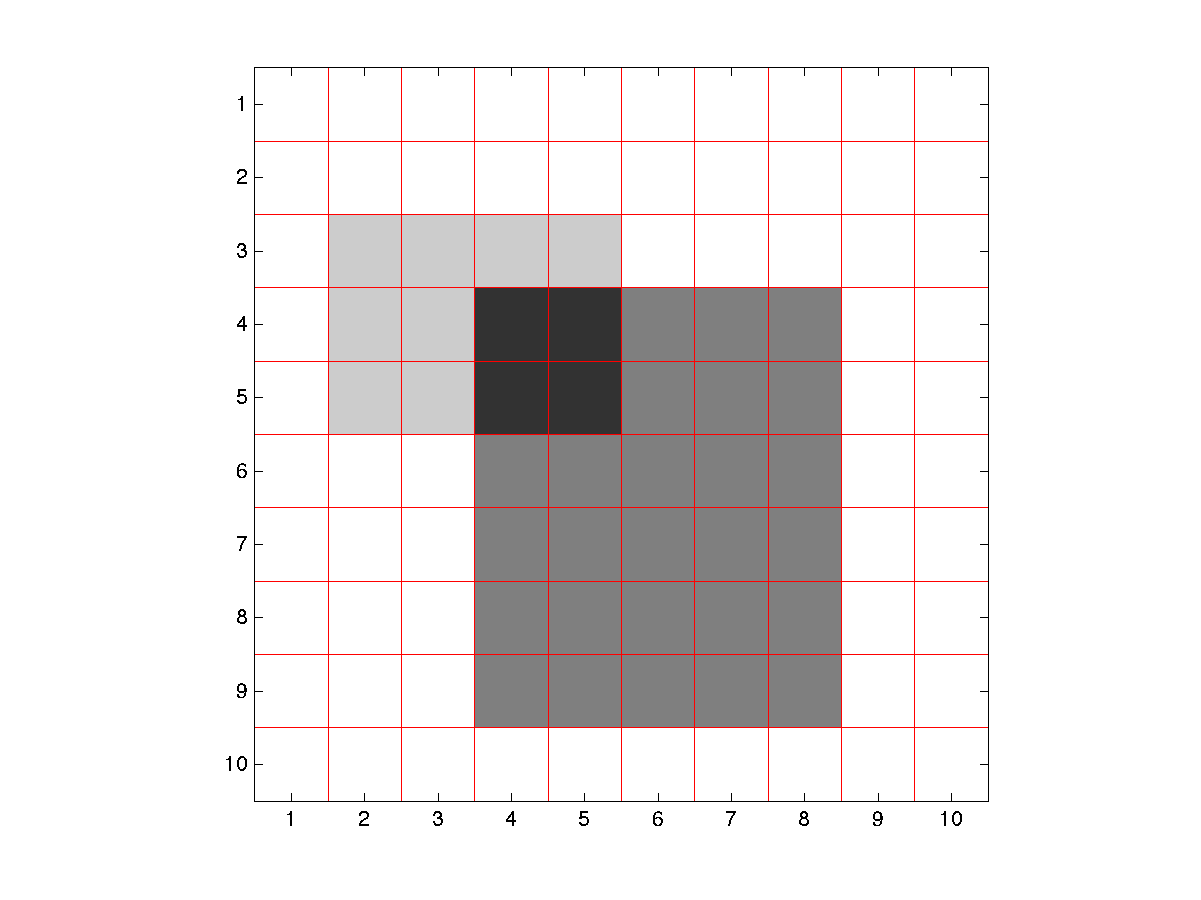
\includegraphics[width=3.5in]{image1.png}}

In Matlab, if $C$ is defined to be the $10 \times 10$ matrix above, then the
commands below will produce this plot (see the end of the assignment for a
Python version):

\begin{verbatim}
cmap = linspace(1,0,11)' * [1 1 1];   % define grayscale colormap
figure
colormap(cmap)     % use gray scale colormap
image(11*C)        % plot image (indexing into colormap of length 11)

hold on    % now add grid lines for clarity...
x = linspace(0.5,10.5,11);
y = x;
[X,Y] = meshgrid(x,y)
plot(X',Y','r')    % plot horizontal grid lines
plot(X,Y,'r')      % plot vertical grid lines
axis square        % scale x and y axis equally
hold off
\end{verbatim} 

Note that we scale $C$ by 11 to index into the colormap which is defined here
as an $11 \times 3$ matrix with {\tt [R,G,B]} values corresponding to 11
shades of gray.  (Note that this matrix has been specified as an outer product
of a column vector with 11 components and a row vector with 3 components.
Print these things out if you are not sure what this matrix looks like.)

The matrix $C$ given above can also be specified fairly easily as a
combination of two outer products, $C = 0.3a_1b_1^T + 0.6a_2b_2^T$ where
for example $a_1 = [0,0,1,1,1,0,0,0,0,0]^T$ and $b_1 =
[0,1,1,1,1,0,0,0,0,0]^T$. 

{\bf Problem 5a.} Compute the matrix $A_1 = a_1b_1^T$ and produce a plot of the image
that this describes.  

{\bf Problem 5b.} Determine the vectors $a_2,~ b_2$ and the matrix $A_2 = a_2b_2^T$
so that the matrix above can be written as $A = 0.3A_1 + 0.6A_2$.  

Note that it takes much less storage to store the image in terms of the
vectors forming these outer products than it would to store every element of
the matrix.  This would be more dramatic if the image were say $1000 \times
1000$ (1 megapixel, with 1,000,000 matrix elements) rather than only
$10\times 10$.  This is a form of image compression. 

This works so well because the matrix for this image is a rank 2
matrix and so only 2 outer products are needed.  If it were a full
rank matrix then this compression might not work so well. But images
generally aren't random pixels.  Instead they have a lot of structure
and so it is sometimes possible to approximate an image well with
a low rank approximation.

The singular value decomposition gives a way of writing any matrix 
as a linear combination of rank one matrices (outer products) and if the
singular values decay rapidly (which they often do for real images) then we
may be able to truncate the SVD to relatively few terms. 

{\bf Problem 5c.} Use Matlab or Python to determine the SVD of the matrix $A$ above
and confirm that only two singular values are nonzero.  With this
decomposition we see that we can express $C$ as $C = \sigma_1 u_1v_1^* +
\sigma_2 u_2 v_2^*$.  Confirm that this is true and print out the singular
values and vectors used in this sum, and also the two
rank-1 matrices that appear in this sum separately.  

{\bf Problem 5d.} Plot the image given by the matrix $\sigma_1 u_1v_1^*$.  This is
the best approximation to the matrix $C$ by a rank-1 matrix.  

{\bf Problem 5e.} Confirm that $u_1$ and $u_2$ are orthonormal vectors
(whereas $a_1$ and $a_2$ were not).  In fact $u_1$ and $u_2$ form an
orthonormal basis for the 2-dimensional space $\text{span}(a_1,a_2)$.
To check this: In Matlab (or Python), form the matrix 
with columns $[u_1 | u_2 | a_1 | a_2]$ and confirm that it has rank 2.
Explain why this shows that the vectors $u_1$ and $u_2$ span the same
subspace of $\complex^2$ as that spanned by $a_1$ and $a_2$.

\vskip 5pt
{\bf Note:} The SVD is not the best approach for image compression,
and the point of this example is primarily to get familiar with the
SVD and the idea of low-rank representations of a matrix.

See
\url{https://www.mathworks.com/company/newsletters/articles/professor-svd.html}
for an introductory article by Cleve Moler (inventor of Matlab) on
the SVD that also shows an example of using it to compress an image
of Gene Golub, who did much to popularize the use of the SVD for a
wide range of applications.  

\vskip 1cm
{\bf Plotting an image in Python:}

This produces a similar plot to the one shown above, but flipped vertically
and also recall that Python indexing starts at 0.

\begin{verbatim}

imshow(C, cmap='Greys', interpolation='none')
x = linspace(-0.5,9.5,11)
y = x
[X,Y] = meshgrid(x,y)
plot(X.T,Y.T,'r');
plot(X,Y,'r');
axis('scaled')
axis([-0.5, 9.5, -0.5, 9.5])
\end{verbatim} 

\end{document}

